\chapter{MÔ PHỎNG THỰC NGHIỆM}

\section{Lựa chọn bài toán}

Nghiên cứu chọn bài toán \textbf{Hoán vị} làm đối tượng thực nghiệm chính với các lý do:
\begin{itemize}
    \item \textbf{Độ phức tạp tập hợp thấp hơn:} So với phép cộng và nhân, phép hoán vị có $C_i = 0$ (không có tương quan không mong muốn), dẫn đến tỷ lệ $\sigma^2/\mu^2$ nhỏ hơn
    \item \textbf{Tài nguyên tính toán:} Kích thước tập hợp các mô hình cần thiết nằm trong khả năng của phần cứng hiện có
    \item \textbf{Tính đại diện:} Mặc dù đơn giản hơn, hoán vị vẫn đủ để chứng minh tính đúng đắn của lý thuyết về tập kết hợp nhiều mô hình và khả năng đạt độ chính xác tuyệt đối
\end{itemize}

\section{Bài toán Hoán vị}

\textbf{Định nghĩa bài toán:}
Cho hoán vị $\pi: [n] \rightarrow [n]$ ngẫu nhiên, mạng nơ-ron được huấn luyện để học ánh xạ này trên các vector cơ sở chuẩn.

\vspace{0.2cm}

\textbf{Thiết lập thực nghiệm:}
\begin{itemize}
    \item \textbf{Tập huấn luyện:} Bao gồm $2n$ mẫu tương ứng với tất cả các ánh xạ vị trí của hoán vị
    \item \textbf{Tập kiểm tra:} 1000 vector kiểm thử được sinh ngẫu nhiên, mỗi vector có $n_{\hat{x}} = 2$ phần tử khác không
    \item \textbf{Độ chính xác:} Được tính là tỷ lệ các vector kiểm tra mà tất cả các bit đầu ra đều đúng sau khi làm tròn
\end{itemize}

\textbf{Điều kiện thành công:}
Vector kiểm tra được coi là đúng nếu và chỉ nếu:
\begin{equation}
    \forall i: \text{sign}(\bar{F}(\hat{\mathbf{x}})_i) = y_i^*
\end{equation}

trong đó $\bar{F}$ là đầu ra trung bình của tập hợp các mô hình.

\section{Độ chính xác theo kích thước của tập hợp các mô hình}

\textbf{Mục tiêu thực nghiệm:}
So sánh số lượng mô hình thực tế cần thiết để đạt độ chính xác mục tiêu (90\%, 95\%, 99\%) với ngưỡng lý thuyết từ Công thức tính số lượng mô hình tối thiểu:
\begin{equation}
    N_{\text{theory}} \geq \frac{2\sigma^2}{\mu^2} \ln\left(\frac{2}{\delta}\right)
\end{equation}

\textbf{Kết quả Thực nghiệm 1:}
\begin{itemize}
    \item Với các giá trị $k$ (kích thước đầu vào thưa) khác nhau, đường độ chính xác thực nghiệm được so sánh với ngưỡng lý thuyết
    \item \textbf{Quan sát chính:} Số lượng mô hình thực tế cần thiết \textbf{luôn nhỏ hơn} ngưỡng chặn lý thuyết
    \item Điều này xác nhận rằng ngưỡng lý thuyết có tính chất bảo thủ, đảm bảo an toàn
\end{itemize}

\textbf{Kết quả Thực nghiệm 2:}
\begin{itemize}
    \item Khi kích thước tập hợp các mô hình tăng lên, độ chính xác tiến dần đến 100\% (độ chính xác tuyệt đối)
    \item Với $k$ lớn hơn, cần nhiều mô hình hơn để đạt cùng mức độ chính xác
    \item Xu hướng này phù hợp với dự đoán lý thuyết: độ phức tạp tập hợp tăng theo $O(k^2)$
\end{itemize}

\begin{figure}[h]
    \centering
    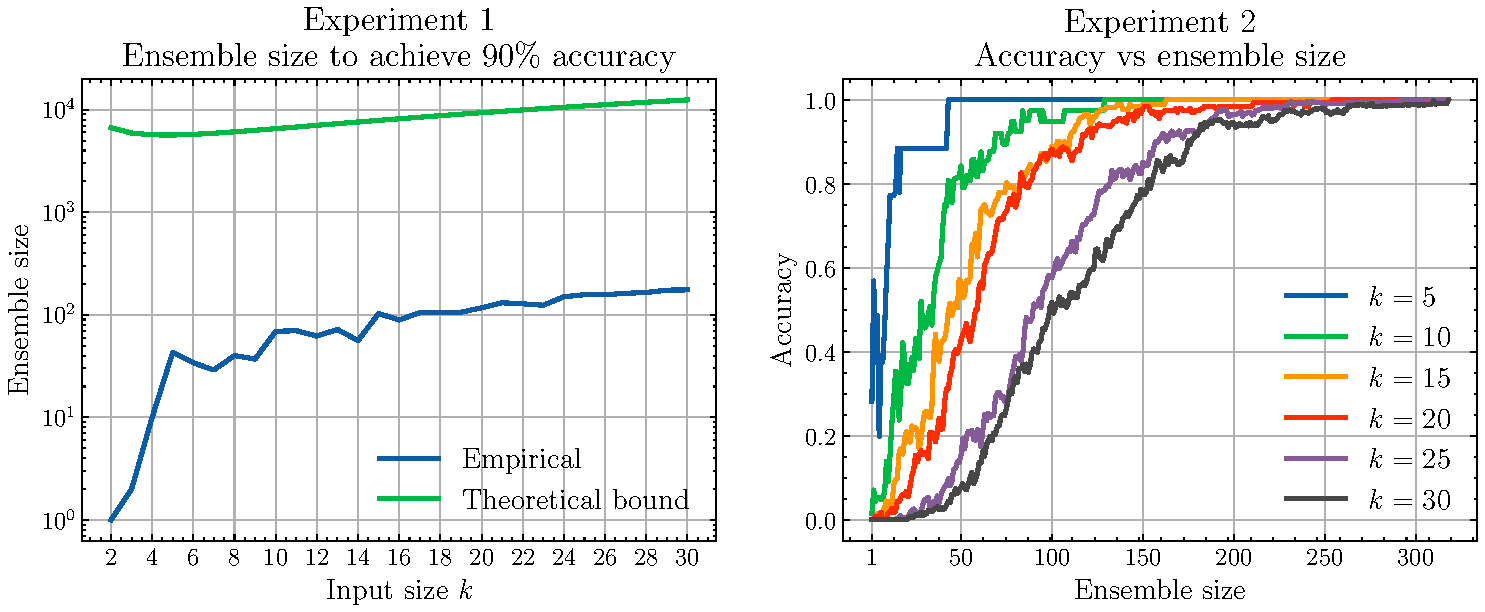
\includegraphics[width=0.9\textwidth]{figures/experiments.pdf}
    \caption{Kết quả thực nghiệm từ bài báo gốc \cite{de_luca_2025}. Thực nghiệm 1 (trái) trình bày số mô hình cần thiết để đạt độ chính xác 90\% theo kích thước đầu vào $k$, so sánh với ngưỡng lý thuyết từ công thức tính số lượng mô hình tối thiểu. Thực nghiệm 2 (phải) trình bày độ chính xác theo số mô hình với các kích thước đầu vào $k$ khác nhau.}
    \label{fig:ensemble_experiments}
\end{figure}

\begin{figure}[h]
    \centering

    \begin{subfigure}[t]{0.48\textwidth}
        \centering
        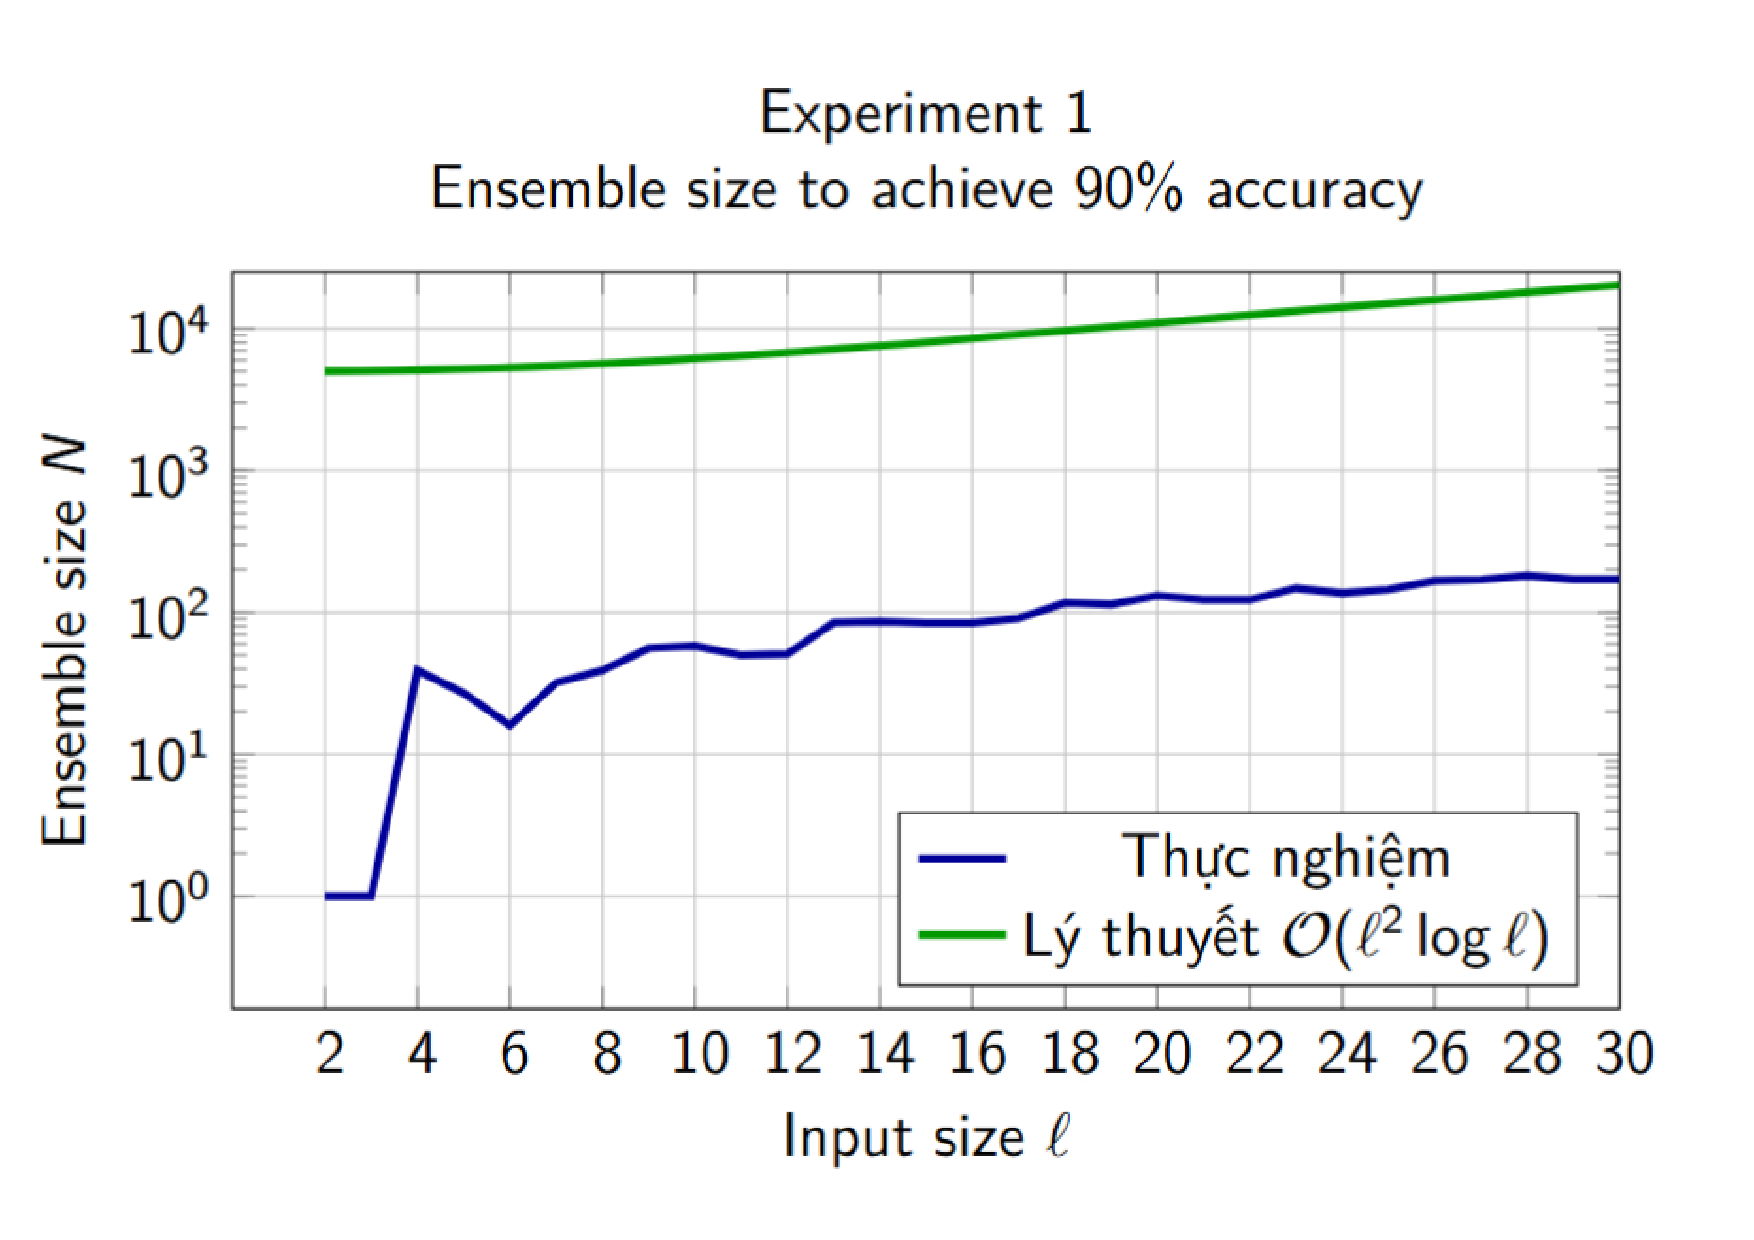
\includegraphics[width=\textwidth]{figures/exp1.pdf}
        \label{fig:exp1}
    \end{subfigure}
    \hfill
    \begin{subfigure}[t]{0.48\textwidth}
        \centering
        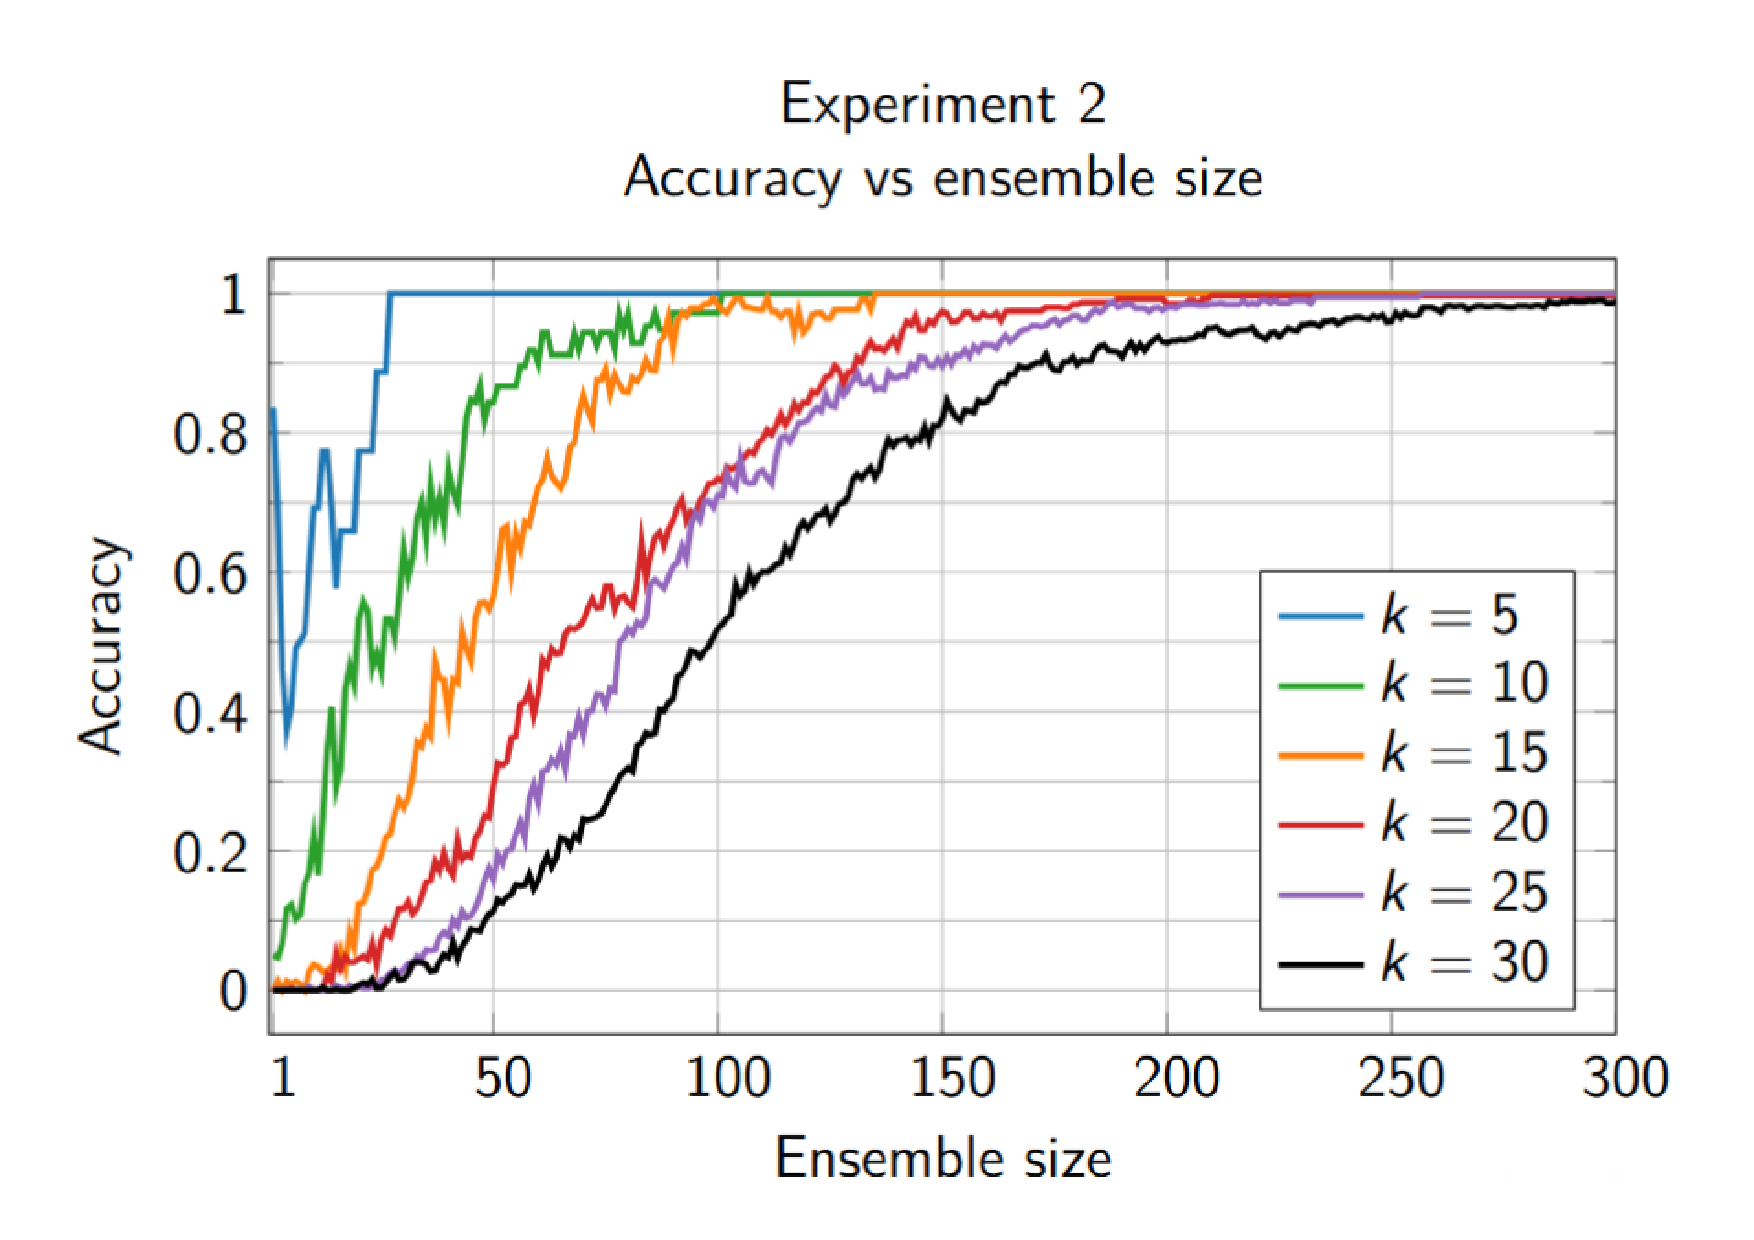
\includegraphics[width=\textwidth]{figures/exp2.pdf}
        \label{fig:exp2}
    \end{subfigure}

    \caption{Kết quả nhóm thực nghiệm lại các thí nghiệm trong bài báo.}
    \label{fig:my_experiments}
\end{figure}


\section{Phân tích kết quả}

Các kết quả phân tích cho thấy ba điểm chính:

\begin{enumerate}
    \item \textbf{Sự phù hợp về dạng hàm:} Hàm thực nghiệm có hình dạng tương đồng với hàm lý thuyết. Điều này xác nhận rằng thực nghiệm tăng trưởng đúng theo quy luật mà lý thuyết đã dự báo.
    
    \item \textbf{Tính bảo thủ của ngưỡng lý thuyết:} Ngưỡng chặn lý thuyết được xây dựng dựa trên các bất đẳng thức tập trung cho biến ngẫu nhiên Gaussian và kỹ thuật \textit{union bound} (trường hợp xấu nhất). Do đó, ngưỡng này luôn đảm bảo tính an toàn và là chặn trên chặt chẽ cho thực tế.

    \item \textbf{Tính khả thi thực tiễn:} Vì số lượng mô hình chỉ tăng theo hàm đa thức nên việc triển khai là hoàn toàn khả thi. Trong thực tế, các phân phối thường tốt hơn giả định xấu nhất và các sai số có thể triệt tiêu lẫn nhau, dẫn đến số lượng mô hình cần thiết nhỏ hơn đáng kể so với lý thuyết.
\end{enumerate}

\section{Thực nghiệm với bài toán Cộng nhị phân}

Ngoài bài toán hoán vị, nhóm cũng tiến hành thực nghiệm với bài toán cộng nhị phân để đánh giá khả năng mở rộng của phương pháp đề xuất.

\vspace{0.2cm}

\textbf{Thiết lập thực nghiệm:}
\begin{itemize}
    \item \textbf{Bài toán:} Cộng hai số nhị phân $k$-bit với $k = 2$.
    \item \textbf{Chiều rộng lớp ẩn:} $n_h = 50,000$ (giống các thực nghiệm trước).
    \item \textbf{Kích thước ensemble:} Thay đổi từ 1 đến 300 mô hình.
    \item \textbf{Tập kiểm tra:} 1000 cặp số ngẫu nhiên.
\end{itemize}

\vspace{0.2cm}

\textbf{Kết quả quan sát:}

Khi tăng kích thước ensemble từ 1 đến 300 mô hình, độ chính xác \textbf{gần như không thay đổi} và duy trì ở mức rất thấp. Cụ thể:
\begin{itemize}
    \item Với 1 mô hình: Độ chính xác đạt khoảng 8-10\%.
    \item Với 150 mô hình: Độ chính xác đạt khoảng 10\%.
    \item Với 300 mô hình: Độ chính xác \textbf{vẫn chỉ duy trì ở mức 10\%}.
\end{itemize}

Kết quả này cho thấy với cấu hình phần cứng hiện tại, bài toán cộng nhị phân đòi hỏi \textbf{yêu cầu tính toán nặng hơn đáng kể} so với bài toán hoán vị để đạt được độ chính xác cao.

\textbf{Phân tích nguyên nhân:}

\begin{enumerate}
    \item \textbf{Chiều rộng lớp ẩn không đủ lớn:}
    
    Lý thuyết NTK dựa trên giả định rằng chiều rộng lớp ẩn $n_h \rightarrow \infty$. Trong thực tế, với $n_h = 50,000$, mạng vẫn hoạt động trong chế độ \textit{chiều rộng vô hạn} thay vì chế độ NTK lý tưởng.
    
    Với bài toán cộng, số lượng tương quan không mong muốn $C_i \leq 1$, cao hơn so với hoán vị ($C_i = 0$). Điều này dẫn đến:
    \begin{itemize}
        \item Tỷ lệ $\sigma^2/\mu^2$ lớn hơn, yêu cầu nhiều mô hình hơn để triệt tiêu phương sai.
        \item Hiệu ứng chiều rộng vô hạn trở nên đáng kể hơn, làm sai lệch dự đoán của bộ dự báo NTK so với mạng thực tế.
    \end{itemize}
    
    \item \textbf{Giới hạn phần cứng:}
    
    Việc tăng chiều rộng lớp ẩn để tiệm cận chế độ NTK lý tưởng bị hạn chế bởi tài nguyên tính toán:
    \begin{itemize}
        \item \textbf{Bộ nhớ GPU:} Mỗi mô hình với $n_h = 50,000$ tiêu tốn đáng kể bộ nhớ. Việc tăng $n_h$ lên 100,000 hoặc cao hơn vượt quá khả năng của GPU hiện có.
        \item \textbf{Thời gian huấn luyện:} Với ensemble gồm 300 mô hình, thời gian huấn luyện tổng cộng đã lên đến nhiều giờ. Việc tăng $n_h$ sẽ làm tăng thời gian này theo bậc hai.
        \item \textbf{Tính toán ma trận NTK:} Với bài toán cộng, kích thước ma trận kernel tăng nhanh theo số bit, làm tăng chi phí tính toán nghịch đảo ma trận.
    \end{itemize}
\end{enumerate}

\section{Kết luận từ thực nghiệm}

Kết quả thực nghiệm cho thấy khoảng cách giữa lý thuyết và thực tiễn trong việc triển khai khung NTK. Mặc dù lý thuyết đảm bảo độ chính xác tuyệt đối với điều kiện $n_h \rightarrow \infty$, việc đạt được điều kiện này trong thực tế đòi hỏi:
\begin{itemize}
    \item Phần cứng tính toán mạnh hơn (GPU với bộ nhớ lớn hơn, hoặc cụm GPU phân tán).
    \item Các kỹ thuật xấp xỉ kernel hiệu quả để giảm chi phí tính toán.
    \item Nghiên cứu thêm về ảnh hưởng của chiều rộng vô hạn đến độ chính xác.
\end{itemize}

Đây là một hướng phát triển quan trọng cho các nghiên cứu tương lai về việc đưa khung lý thuyết NTK vào ứng dụng thực tiễn.

\section{Ý nghĩa thực tiễn}

Kết quả thực nghiệm xác nhận hai điều quan trọng:

\begin{enumerate}
    \item \textbf{Tính đúng đắn của lý thuyết:} Ngưỡng lý thuyết luôn là chặn trên hợp lệ cho số mô hình cần thiết.
    \item \textbf{Khả năng thực tiễn:} Trong ứng dụng thực tế, có thể sử dụng ít mô hình hơn so với ngưỡng lý thuyết mà vẫn đạt độ chính xác cao (như đã thấy trong bài toán hoán vị).
\end{enumerate}
